
\section{Experimental Setup}
\label{sec:setup}




\begin{figure*}
 
    \begin{multicols}{2}
    %\begin{minipage}
    %\resizebox{\columnwidth}{!}{
    \begin{subfigure}{0.45\textwidth}
    
\begin{tikzpicture}
\begin{axis}[
    xlabel={\textbf{Number of Flows}},
    ylabel={\textbf{Throughput}},
    xtick=data,
    legend pos=north west]
    \addplot[mark=diamond*,thick,red] coordinates {
        (100, 304.9)
(200, 548.197)
(300, 733.797)
(400, 911.396)
(500, 1011.883)
(600, 1122.26)
(700, 1190.12)
(800, 1285.59)
(900, 1345.2)
(1000, 1403.6)
} node[pos=0.7,below,anchor=west];
    
    \addplot[mark=x,mark options={solid},blue,thick,dashed] coordinates {
(100, 295.7)
(200, 490.9)
(300, 659.7)
(400, 790.689)
(500, 871.11)
(600, 961.77)
(700, 1023.12)
(800, 1109.215)
(900, 1165.7)
(1000, 1211.51)
}node[pos=0.7,above,anchor=east];


    \addplot[mark=o,mark options={solid},green,thick, dashed] coordinates {
(100, 304.9)
(200, 581.4)
(300, 717.19)
(400, 756.8)
(500, 765.1)
(600, 765.1)
(700, 798.8)
(800, 794.2)
(900, 776.4)
(1000, 787.75)
}node[pos=0.7,above,anchor=east];


    \addplot[mark=o,mark options={solid},black,thick,dashed] coordinates {
(100, 304.9)
(200, 588.2)
(300, 892.38)
(400, 1182.7)
(500, 1498.9)
(600, 1813.26)
(700, 2109.3)
(800, 2420.2)
(900, 2742.2)
(1000, 3056.5)
}node[pos=0.7,above,anchor=east];



\legend{PDA($\epsilon$=0.5),PDA($\epsilon$=0.75), RA-RA, Upper Bound}
\end{axis}
\end{tikzpicture}
\caption{Throughput for Fat-Tree topology}
\label{fig:sub1}
 \end{subfigure}\hspace{8mm}
% \end{minipage}

% \begin{minipage}
    \begin{subfigure}{0.45\textwidth}
    \begin{tikzpicture}
    \begin{axis}[
        xlabel={\textbf{Number of Flows}},
    ylabel={\textbf{Throughput}},
    xtick=data,
    legend pos=north west]
        \addplot[mark=o,mark options={solid},blue,thick,dashed] coordinates {
        (50, 145.191)
(100, 304.9)
(200, 588.297)
(300, 764.896)

}node[pos=0.7,above,anchor=east];
    
            \addplot[mark=o,mark options={solid},black,thick,dashed] coordinates {
        (50, 145.191)
(100, 304.9)
(200, 588.297)
(300, 892.38)

}node[pos=0.7,above,anchor=east];

    
    \legend{TMA, Upper Bound}
\end{axis}
\end{tikzpicture}
\caption{Throughput for TMA in Fat Tree Topology}
\label{fig:sub2}
    \end{subfigure}
    \end{multicols}
    
%%%%%%%%%%%%%%%%%%%%%%%%CORONA TOPOLOGY%%%%%%%%%%%%%%%%%%%%%%%%%%
    \begin{multicols}{2}
    \begin{subfigure}{0.45\textwidth}
    
\begin{tikzpicture}
\begin{axis}[
    xlabel={\textbf{Number of Flows}},
    ylabel={\textbf{Throughput}},
    xtick=data,
    legend pos=north west]
    \addplot[mark=diamond*,thick,red] coordinates {
    
    (100, 304.95) 
(200, 588.29)
(300, 883.89)
(400, 1136.62)
(500, 1347.71)
(600, 1540.79)
(700, 1721.76 )
(800, 1863.39)
(900, 1994.049)
(1000, 2107.62 )

} node[pos=0.7,below,anchor=west];
    
    \addplot[mark=x,mark options={solid},blue,thick,dashed] coordinates {
(100, 304.950)
(200, 588.297)
(300, 852.097)
(400, 1036.900)
(500, 1176.405)
(600,1378.411006353427)
(700, 1522.9892794267275)
(800, 1620.582731192362)
(900, 1706.6110469952177)
(1000, 1797.9923385972693 )
}node[pos=0.7,above,anchor=east];


    \addplot[mark=o,mark options={solid},green,thick, dashed] coordinates {
(100,304.95008052735665)
(200,588.2975326187434)
(300,892.3815061809704)
(400,1089.2800311383057)
(500,1149.5154241140162)
(600,1154.9944623727408)
(700,1213.2833337717482)
(800,1213.7767212368615)
(900,1255.5802839175446)
(1000,1292.8601849607876)

}node[pos=0.7,above,anchor=east];


    \addplot[mark=o,mark options={solid},black,thick,dashed] coordinates {
(100,304.95008052735665)
(200,588.2975326187434)
(300,892.3815061809704)
(400,1182.7698631944063)
(500,1498.9758816081755)
(600,1813.2640738634966)
(700, 2109.33)
(800, 2420.242917993053)
(900,2742.263537968908)
(1000,3056.548111449543)

}node[pos=0.7,above,anchor=east];



\legend{PDA($\epsilon$=0.5),PDA($\epsilon$=0.75), RA-RA, Upper Bound}
\end{axis}
\end{tikzpicture}
\caption{Throughput for CORONET CONUS Topology}
\label{fig:sub3}
 \end{subfigure}\hspace{8mm}
% \end{minipage}

% \begin{minipage}
    \begin{subfigure}{0.45\textwidth}
    \begin{tikzpicture}
    \begin{axis}[
        xlabel={\textbf{Number of Flows}},
    ylabel={\textbf{Throughput}},
    xtick=data,
    legend pos=north west]
        \addplot[mark=o,mark options={solid},blue,thick,dashed] coordinates {
(100, 304.950)
(200, 588.297)
(300, 892.381)
(400, 1182.769)


}node[pos=0.7,above,anchor=east];
    
            \addplot[mark=o,mark options={solid},black,thick,dashed] coordinates {
(100,304.95008052735665)
(200,588.2975326187434)
(300,892.3815061809704)
(400,1182.7698631944063)


}node[pos=0.7,above,anchor=east];

    
    \legend{TMA, Upper Bound}
\end{axis}
\end{tikzpicture}
\caption{Throughput for TMA in CORONET CONUS Topology}
\label{fig:sub4}
    \end{subfigure}
    
    \end{multicols}
    
    
    %\end{minipage}
    %}
    
\caption{Performance in terms of network throughput for TMA, PDA and RA-RA over different topologies.}

    \label{fig:graph}
\end{figure*}


In this section we explain the platform, topologies, configuration we used for our experiment. As we were not bench marking the time and resource utilization of the algorithms, we ran our experiments on CloudLab, Amazon Web Services and Local Desktop and collaborated the results. These experiments can be found in \cite{ref:gitimpl}.

\subsection{Platform}
We initially planned to implement our routing algorithms in NS3, OPNET or Java Network Simulator. This would have helped us see graphical simulation of the network. At the same time, we would have needed to setup the complete environment and team would have required to learn new technologies.  As we moved ahead with studying different algorithms, we realized that we do not need a graphical simulation of the network to benchmark throughput and it will be a waste of effort to invest time in learning network simulation languages like Tcl, ns2 etc.  The algorithms find path to route the flows using Dijkstra and breadth first search and satisfy the required constraints using linear programming. Between MATLAB and Python, Python seemed more intuitive because of the availability of wide community support, inbuilt libraries for solving linear programming and flexibility of the language. Solving all the constraints, we finalized \textbf{Python Language and Env} for implementing the algorithms and running the experiments. 

\subsection{Topologies}
Network topologies can have a substantial effect on 
performance of the algorithm or network topology plays an important role in choosing the correct algorithm for network routing. \cite{ref:paper1} solve PDA and TMA algorithms, perform experiment on FAT-Tree and GEANT Topology where as the RA-RA algorithm \cite{ref:paper2} uses to CORONET CONUS topology to perform the experiments. To have a fair comparison, we use the FAT-TREE topology from the work on PDA and TMA in \cite{ref:paper1}  and CORONET CONUS topology from RA-RA proposed in ~\cite{ref:paper2} to do the comparative study. 

\subsubsection{Fat-Tree}
The Fat-Tree topology  ~\cite{ref:fat-tree} is a tree branch topology with a core layer, aggregation layer, edge layer and hosts. For our experiment, we had 16 Core Switches, 32 Aggregation Switches, 32 Edge Switches and 128 hosts. There are 8 different types of Virtual functions deployed on 24 function nodes. The function nodes are deployed on switches as separate machines(not the node itself). Each type has 3 middle boxes deployed randomly on the nodes of the fat tree.  
The capacities(bandwidth) of link in the Fat-Tree are as follows: 

1. 200 units/link between core and aggregation layer.

2. 100 units/link between aggregation layer and edge layer.

3. 100 units/link between edge and host layer. 

Each middle box is connected to the switch using a link with capacity 200 units. The processing power of the middle boxes is limited to 300 units. 

\subsubsection{CORONET CONUS}
\begin{figure}[ht]
\vskip 0.2in
\begin{center}
\centerline{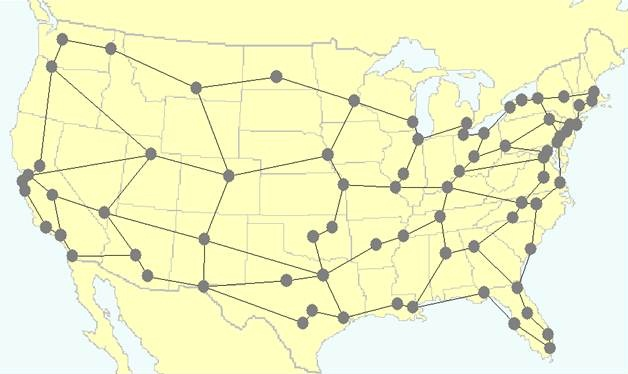
\includegraphics[width=\columnwidth]{Report//graphs/coro.jpg}}
\caption{CORONET CONUS Topology ~\cite{ref:coronus}}
\label{pruning}
\end{center}
\vskip -0.2in
\end{figure}
This topology is a real world topology between different cities in the United State of America ~\cite{ref:coronus}. It consists of 60 Nodes and 79 links. In our experiment, each link in the network has a capacity(bandwidth) of 1000 units. The VNFs are deployed on top 30\% of the nodes based on the degree of the nodes. There are a total of 20 Virtual Network Functions. Each function node, hosts 8 different types of virtual network functions. Therefore, 18 nodes each with 8 different types of virtual network functions gives a total of 144 Virtual Network Function deployments across the network. Since many virtual network functions are deployed on a single node, the processing capacity of each functional node was kept to be 1000 units. 

\subsection{Experiment Configuration}
In this section, we will discuss about the different configurations and constraints we removed or added in each experiment make the comparison fair. 

\subsubsection{Comparison on Fat-Tree}
Our first experiment was on Fat-Tree topology. The flows were generated randomly from source and destination chosen from hosts in the Fat-Tree topology. The number of virtual network functions required by a particular flow request can be up to 6. Also, for RA-RA flows with less than 2 units capacity are considered mice flows and are given high priority.  To make the comparison fair, we assume that each flow takes equal bandwidth over all the links. The capacity of each flow is assigned randomly  between 1 and 5 units. Similarly it is assumed that each flow uses the same capacity for every middlebox function and is randomly assigned between 1 and 4 units. 

\subsubsection{Comparison on CORONET CONUS}
In our second experiment on CORONET CONUS topology, the flows were generated in a different manner. The source and destination nodes could be any of the nodes in the network and are chosen randomly for a given flow. Also, setting the number of VNFs required by a flow to 6 was consuming a lot of processing power on all the platforms (CloudLab, AWS and Local Desktop). We therefore limited the number of Virtual Network Functions in a flow request to 3, thus limiting the length of each flow to 5. The bandwidth usage was assigned a value between 1 and 5 units and for the functional node, a value between 1 and 4 units similar to Fat-Tree topology.
